\subsection{ATAC-sequencing and CTCF sequencing}
ATAC-sequencing is a technology that allows for the identification of open chromatin regions 
\cite{buenrostroTranspositionNativeChromatin2013a, grandiChromatinAccessibilityProfiling2022}. 
In order to work, it requires the addition of TN-5, a hyper-active transposase. The latter is preloaded with sequencing adapters
\cite{grandiChromatinAccessibilityProfiling2022}
to induce a contempourary reaction of fragmentation and ligation of the pieces released, in a process called segmentation. The obtained adapted fragments are then amplified and sequenced. Once the reads are generated, a peak-calling algorithm (generally MACS-2 
\cite{zhangModelbasedAnalysisChIPSeq2008a}) 
is used to determine which portions of the genome present ATAC peaks, and areas where there are significant enrichments of aligned reads with respect to the background. A significant enrichment of reads is possible only in accessible regions, which are generally also the most active ones and with available sites for transcription factors binding. The CTCF data used for this experiment, named in table \ref{tab:data}, were obtained through a classical ChIP-sequencing, which is a method that combines chromatin immunoprecipitation with DNA sequencing to infer the possible binding sites of DNA-associated proteins (consult the ENCODE entry in table \ref{tab:data} for more information).


\begin{figure}[H]
    \centering
    
    \begin{subfigure}{0.69\textwidth}
      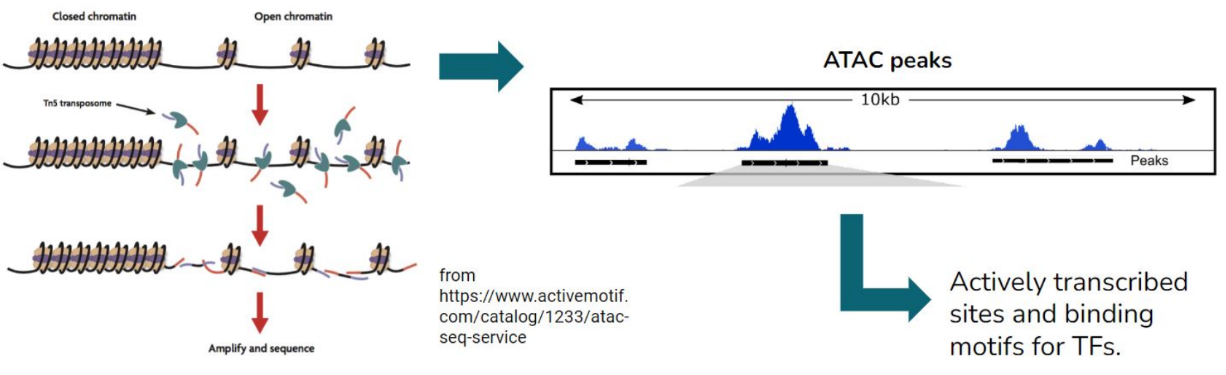
\includegraphics[width=\linewidth]{./ATAC_sequencing.png}
      \caption{Basic concept behind the ATAC-sequencing technique. The images were taken from the following \href{https://www.activemotif.com/catalog/1233/atac-seq-service}{link}.}
      \label{fig: ATAC-sequencing}
    \end{subfigure}
    \hfill
    \begin{subfigure}{0.30\textwidth}
      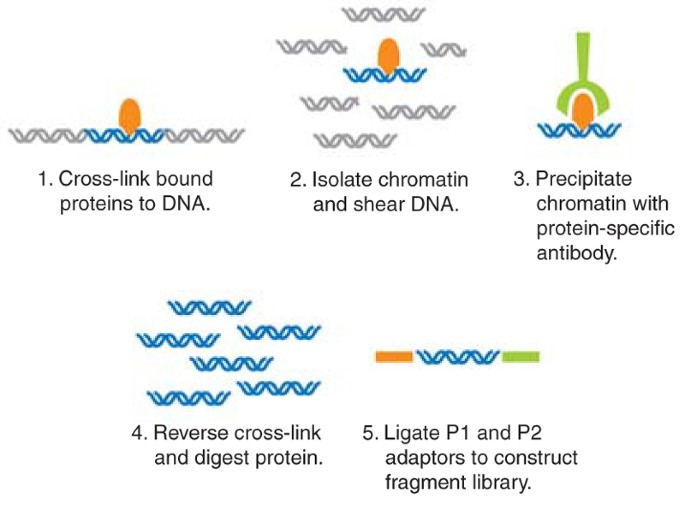
\includegraphics[width=\linewidth]{./ChIP-Seq_procedure.png}
      \caption{Pipeline to perform a generic ChIP-sequencing analysis. The image was taken from the work of Anjali Shah\cite{shahChromatinImmunoprecipitationSequencing2009}.}
      \label{fig: CTCF ChIP-Seq}
    \end{subfigure}
  
    \caption{}
    % \label{fig:}
\end{figure}
